\documentclass[a4paper]{article} 
\usepackage{geometry,fancyhdr,caption,subcaption,graphicx,psfrag,amsfonts,textcomp,mathtools,amsmath,hyperref} 

% settings courtesy of http://www.tjansson.dk/?p=419
\usepackage{listings}
\usepackage{color}
\usepackage{textcomp}
\definecolor{listinggray}{gray}{0.9}
\definecolor{lbcolor}{rgb}{0.9,0.9,0.9}
\lstset{
	backgroundcolor=\color{lbcolor},
	tabsize=4,
	rulecolor=,
	language=matlab,
        basicstyle=\scriptsize,
        upquote=true,
        aboveskip={1.5\baselineskip},
        columns=fixed,
        showstringspaces=false,
        extendedchars=true,
        breaklines=true,
        prebreak = \raisebox{0ex}[0ex][0ex]{\ensuremath{\hookleftarrow}},
        frame=single,
        showtabs=false,
        showspaces=false,
        showstringspaces=false,
        identifierstyle=\ttfamily,
        keywordstyle=\color[rgb]{0,0,1},
        commentstyle=\color[rgb]{0.133,0.545,0.133},
        stringstyle=\color[rgb]{0.627,0.126,0.941},
}

\title{Mandatory exercise 7 \\
Signal and Image Processing 2012} 
\author{Jens P. Raaby \\
\url{frn617@diku.dk}}

\begin{document} 
\maketitle

\section{Development of the compression method, including reasons for choices}
\subsection{Encoding}
I first considered the steps that encoding would involve. Gonzalez \& Woods suggest the compression is first a mapping stage, then a quantizing stage, then a symbol coding stage. This latter stage is designed to simply remove the redundant information and minimise the storage required. It can therefore be implemented as a lossless encoding step. One simple option would be to use the zip compression on the binary data, effectively offloading the compression to another algorithm. Since that is not in the spirit of this assignment, I considered the methods presented in the textbook for losslessly coding binary data. Huffman coding is a traditional choice and is often used in JPEG encoders, and my initial attempts at compression involved implementing a huffman dictionary as a Matlab cell array. This required a lot of code and was not very elegant, so I decided to use the Matlab toolbox huffman functions with my own symbols used to create the dictionary.

I also considered arithmetic coding which is a more modern method for removing redundant information. 

\subsection{Decoding}


\section{Reasons for choices (WHY I DID IT THAT WAY)}
\subsection{Types of redundancy, possible solutions, choices}
\begin{itemize}

    \item Coding redundancy


    \item Spatial redundancy


    \item Irrelevant information
\end{itemize}

\subsection{Options for storing parameters}

\section{Analysis of the results on the lena.bmp image}
\begin{itemize}

    \item reconstructed image

    \item SNR

    \item Comp ratio
\end{itemize}

\subsection{Properties of the Lena Image}


\section{Discussion of the results in general - potential improvements}

% \begin{figure}
%     
%         \centering
%         \begin{subfigure}[b]{0.4\textwidth}
%                 \centering
%                 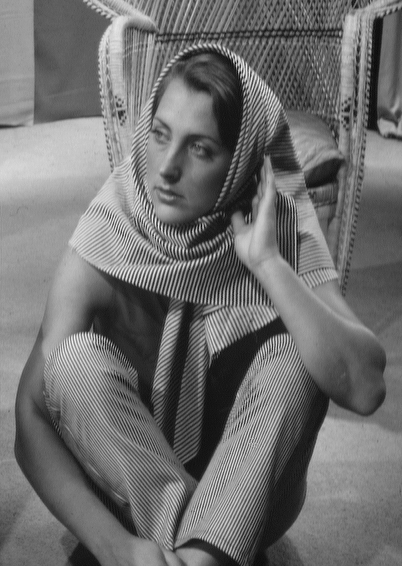
\includegraphics[width=\textwidth]{q4-orig.png}
%                 \caption{The Original IC.tif image}
%                 \label{fig4:orig}
%         \end{subfigure}
%         \begin{subfigure}[b]{0.4\textwidth}
%                 \centering
%                 \includegraphics[width=\textwidth]{q4-denoised.png}
%                 \caption{The denoised image}
%                 \label{fig4:denoise}
%         \end{subfigure}
%         
%         \caption{Decomposed signals}        
%         \label{fig4}
% \end{figure}

\clearpage
\% appendix 
% \section{Question 6.3 source} 
% \label{appendix-lst3} 
% \lstinputlisting{q63.m}
% \section{Question 6.4 source} 
% \label{appendix-lst4} 
% \lstinputlisting{q64.m}
\end{document} 
